%Suitability of Exciters for Perceptual Control
%	Parameterise feature changes in terms of harmonic excitation.
%	Most suitable methods for given feature manipulations.
%	Easiest features to control in isolation.

\chapter{Controlling Audio Features} % control of low level features using exciters
\label{chap:FeatureControl}

\section{Introduction}
\label{sec:FeatureControl-Introduction}
	As discussed in Section \ref{sec:Timbre-Control}, previous studies have attempted to control perceptual features by 
	controlling specific audio features. This chapter will identify the audio features which can be controlled through 
	harmonic excitation and which excitation algorithms are the most suitable for given feature changes. 

\section{Parameterisation of Feature Changes}
\label{sec:FeatureControl-Parameterisation}
	This section discusses the parameterisation of various audio features. The measurement of each audio feature is
	discussed and methods by which a single parameter can be used to adjust them are suggested.

	Several of the audio features discussed involve analysis of a signals spectrum. To simplify the notation of these
	features it is useful to introduce the concept of a spectral component. A spectral component describes a part of the
	signals spectrum, be it a spectral bin obtained from a DFT, a partial of the signal, or a frequency band taken from
	the spectrum. In the following equations, unless otherwise stated, the symbols $a_{n}$ and $\nu_{n}$ will refer to
	the amplitude and frequency of the $n$\super{th} spectral component of a signal respectively.

	\subsection{Spectral Moments}
	\label{sec:FeatureControl-Parameterisation-SpectralMoments}
		\subsubsection*{Spectral Centroid}
			The spectral centroid of a signal, $\mu$, is the first raw moment (mean) of the spectrum. It is
			calculated using Equation \ref{eq:SpectralCentroid}.

			\begin{equation}
				\mu = \frac{\sum_{n = 1}^{N} \nu_{n}a_{n}}
				           {\sum_{n = 1}^{N} a_{n}}
				\label{eq:SpectralCentroid}
			\end{equation}

			Where $N$ is the number of spectral components.

			A crude method of causing $\mu$ to move towards a particular frequency is the increase the energy at
			that frequency. While this works conceptually it is destructive to the original structure of the
			spectrum. As $\mu$ moves towards the desired frequency the spectrum is dominated by a sinusoid at
			that frequency.

			Less destructive methods include that used by \citet{zacharakis2011an} who split the signal into two
			bands, one above and one below the spectral centroid. The relative amplitudes of these bands can
			then be altered to adjust the spectral centroid. This preserves more of the original signals
			structure, the relative levels of partials within each band remaining the same. Using this method
			the new spectral centroid will lie somewhere between the respective centroids of the two bands. The
			relative amplitudes of the two bands required to give a certain spectral centroid, $\mu$, can be
			calculated using Equation \ref{eq:SpectralCentroidManipulation}.

			\begin{equation}
				\frac{\sum_{n = c + 1}^{N} a_{n}}
				     {{\sum_{n = 0}^{c} a_{n}}} = 
				\frac{\mu_{l} - \mu}{\mu - \mu_{u}}, 
				\quad \mu_{l} \leq \mu < \mu_{u} \quad \textrm{or} \quad \mu_{u} < \mu \leq \mu_{l}
				\label{eq:SpectralCentroidManipulation}
			\end{equation}

			Where $\mu_{l}$ and $\mu_{r}$ are the spectral centroid of the upper and lower band, and $c$ is the
			order highest frequency spectral component in the lower band.

			\citet{williams2007perceptually} employ a spectral tilt to manipulate spectral centroid, applying
			gain to the partials of a signal as a linear function of their frequency. This allows the spectral
			centroid to be moved up or down in frequency while still retaining the frequency content of the
			signal. A disadvantage of this method is that the change in centroid cannot be easily parameterised
			as it depends on the content of the signal being processed.

			Another way to move the spectral centroid is by introducing a new band of energy into the spectrum.
			This is conceptually similar to the two band method discussed previously but allows the second band
			to contain frequency content which was not in the original signal. As before the overall spectral
			centroid can be moved by adjusting the relative amplitudes of the original signal and the new band
			of energy. This method also proved difficult to parameterise as destructive superposition could
			occur between the partials of the two signals being summed.

		\subsubsection*{Spectral Spread}
			The spectral spread of a signal, $\sigma^{2}$, is the second central moment (variance) of the
			spectrum. It is calculated using Equation \ref{eq:SpectralSpread}.

			\begin{equation}
				\sigma^{2} = \frac{\sum_{n = 1}^{N} a_{n}(\nu_{n} - \mu)^{2}}
				                  {\sum_{n = 1}^{N} a_{n}}
				\label{eq:SpectralSpread}
			\end{equation}

		\subsubsection*{Spectral Skewness}
			The spectral skewness of a signal, $\gamma$, is the third standardised moment of the spectrum. It is
			calculated using Equation \ref{eq:SpectralSkewness}.

			\begin{equation}
				\gamma = \frac{\sum_{n = 1}^{N} a_{n}(\nu_{n} - \mu)^{3}}
					      {\sigma^{3}\sum_{n = 1}^{N} a_{n}}
				\label{eq:SpectralSkewness}
			\end{equation}

		\subsubsection*{Spectral Kurtosis}
			The spectral Kurtosis of a signal, $\kappa$, is the fourth standardised moment of the spectrum. It
			is calculated using Equation \ref{eq:SpectralKurtosis}.

			\begin{equation}
				\kappa = \frac{\sum_{n = 1}^{N} a_{n}(\nu_{n} - \mu)^{4}}
					      {\sigma^{4}\sum_{n = 1}^{N} a_{n}}
				\label{eq:SpectralKurtosis}
			\end{equation}

	\subsection{Tristimulus}
	\label{sec:FeatureControl-Parameterisation-Tristimulus}
		The three tristimulus metrics can be calculated using Equations \ref{eq:Tristimulus1}, \ref{eq:Tristimulus2}
		and \ref{eq:Tristimulus3}.
		
		\begin{equation}
			T_{1} = \frac{h_{1}}{\sum_{n = 1}^{N} h_{n}}
			\label{eq:Tristimulus1}
		\end{equation}

		\begin{equation}
			T_{2} = \frac{h_{2} + h_{3} + h_{4}}{\sum_{n = 1}^{N} h_{n}}
			\label{eq:Tristimulus2}
		\end{equation}

		\begin{equation}
			T_{3} = \frac{\sum_{n = 5}^{N} h_{n}}{\sum_{n = 1}^{N} h_{n}}
			\label{eq:Tristimulus3}
		\end{equation}

		Where $h_{n}$ is the amplitude of the $n$\super{th} harmonic in the signal and $N$ the total number of
		harmonics.

		As mentioned in Section \ref{sec:Timbre-LowLevelFeatures-Spectral} each tristimulus metric measures the
		amplitude ratio of a specific set of harmonics and all the harmonics. In each of these equations the
		denominator is always greater than or equal to the numerator. For this reason the tristimulus takes values
		from zero to one. Zero meaning there is no energy in that set of harmonics, one meaning the signal is
		entirely composed of those harmonics.

		A generalised from of these metrics measures the amplitude ratio, $R$, of a specific set of spectral
		components, $S$, and a set which includes that set, $F$. This is shown in Equation
		\ref{eq:GeneralTristimulus}.

		\[ A = \sum_{n \in F} a_{n} \]
		\[ B = \sum_{n \in S} a_{n}, \quad S \subseteq F \]
		\begin{equation}
			R = \frac{B}{A}
			\label{eq:GeneralTristimulus}
		\end{equation}

		This ratio can be adjusted by applying gain to the spectral components in $S$. To attain a particular value
		of $R$ the required gain, $m$, can be calculated using Equation \ref{eq:GeneralTristimulusManipulation}.

		\begin{equation}
			m = \frac{R(B - A)}{B(R - 1)}, \quad 0 \leq R < 1
			\label{eq:GeneralTristimulusManipulation}
		\end{equation}

	\subsection{Odd to Even Harmonic Ratio}
	\label{sec:FetureControl-Parameterisation-HarmonicParityRatio}
		The odd to even order harmonics ratio is calculated using Equation \ref{eq:HarmonicParityRatio}.
		
		\begin{equation}
			R_{\textrm{OE}} = \frac{\sum_{1 \leq n \leq N, n \textrm{ is odd}} h_{n}^{2}}
			              {\sum_{1 \leq n \leq N, n \textrm{ is even}} h_{n}^{2}}
			\label{eq:HarmonicParityRatio}
		\end{equation}

		It describes how much of the signals energy is made up of odd or even order harmonics. This allows for
		distinction between signal which consist only of odd harmonics or of even harmonics. The ration can easily
		be altered by applying gain to the odd harmonics. The required gain factor, $m$, is calculated using
		Equation \ref{eq:HarmonicParityRatioManipulation}.

		\begin{equation}
			m = \sqrt{\frac{R_{\textrm{OE}}\sum_{1 \leq n \leq N, n \textrm{ is even}} h_{n}^{2}}
			               {\sum_{1 \leq n \leq N, n \textrm{ is odd}} h_{n}^{2}}},
				       \quad R_{\textrm{OE}} \geq 0;
		       \label{eq:HarmonicParityRatioManipulation}
		\end{equation}

		Equation \ref{eq:HarmonicParityRatio} produces an asymmetric scale which may be difficult to interpret.
		Signals with most of their energy at even harmonics produce values between zero and one. Signals with more
		energy at the odd harmonics can produce any value greater then one. Another problem arises for signals with
		no energy at even harmonics where a division by zero will occur.

		A more robust measure is to have separate measures for the proportion of odd harmonics in a signal and the
		proportion of even harmonics in a signal.  \citet{lukasik2005towards} describes two metrics which measure
		the oddness, $O$, and the evenness, $E$, of a signal. These are given in Equations \ref{eq:Oddness} and
		\ref{eq:Evenness}.

		\begin{equation}
			O = \sqrt{\frac{\sum_{1 \leq n \leq N, n \textrm{ is odd}} h_{n}^{2}}
			               {\sum_{n = 1}^{N} h_{n}^{2}}}
			\label{eq:Oddness}
		\end{equation}

		\begin{equation}
			E = \sqrt{\frac{\sum_{1 \leq n \leq N, n \textrm{ is even}} h_{n}^{2}}
			               {\sum_{n = 1}^{N} h_{n}^{2}}}
			\label{eq:Evenness}
		\end{equation}

		These both produce values in the range zero to one and satisfy the statement $O + E = 1$. 

		Equations \ref{eq:Oddness} and \ref{eq:Evenness} can be generalised to give Equation
		\ref{eq:GeneralOddness}.

		\[ A = \sum_{n \in F} a_{n}^{2} \]
		\[ B = \sum_{n \in S} a_{n}^{2}, \quad S \subseteq F \]
		\begin{equation}
			R = \sqrt{\frac{B}{A}}
			\label{eq:GeneralOddness}
		\end{equation}

		Like Equation \ref{eq:GeneralTristimulus} this measure the ratio of amplitudes of a set of frequencies and a
		larger set of frequencies. This time using the squares of the amplitudes and taking the square root
		afterwards. The value of the ratio can be altered by applying gain to the spectral components in the set
		$S$. The required gain factor, $m$, is calculated using Equation \ref{eq:GeneralOddnessManipulation}.

		\begin{equation}
			m = \sqrt{\frac{R^{2}(B - A)}{B(R^{2} - 1)}}, \quad 0 \leq R < 1
			\label{eq:GeneralOddnessManipulation}
		\end{equation}

	\subsection{Inharmonicity}
	\label{sec:FetureControl-Parameterisation-Inharmonicity}
		Inharmonicity is a measure of how much the frequencies of a signal's partials deviate from harmonic
		frequencies. This is measured using Equation \ref{eq:Inharmonicity}.
		
		\begin{equation}
			I = \frac{2\sum_{n = 1}^{N}a_{n}^{2}
			           \abs{\nu_{n} - f_{0}\floor{\frac{\nu_{n}}{f_{0}} + \frac{1}{2}}}}
				   {f_{0}\sum_{n = 1}^{N} a_{n}^{2}}
			\label{eq:Inharmonicity}
		\end{equation}

		Where $a_{n}$ and $\nu_{n}$ are the amplitude and frequency of the $n$\super{th} partial in the signal
		respectively and $N$ the total number of partials in the signal.

		This produces values between zero and one. Zero describing a signal in which all partials are harmonics of
		the fundamental and one describing a signal where all partials have frequencies lying
		$\frac{f_{0}}{2}$Hz from harmonic frequencies.

		Controlling the inharmonicity can prove difficult unless certain criteria are met. Consider two signals, $x$
		and $y$, with the same fundamental frequency, which are composed of partials with frequencies in the sets
		$X$ and $Y$ respectively. Provided that $X \medcap Y = \emptyset$ (i.e. $x$ and $y$ have no frequency
		component in common) the inharmonicity of $x + y$ is given by Equation \ref{eq:InharmonicitySum}.

		\begin{equation}
			I = \frac{I_{x}\sum_{\nu \in X} a_{\nu,x}^{2} + I_{y}\sum_{\nu \in Y} a_{\nu,y}^{2}}
			         {\sum_{\nu \in X} a_{\nu,x}^{2} + \sum_{\nu \in Y} a_{\nu,y}^{2}}
			\label{eq:InharmonicitySum}
		\end{equation}

		Where $a_{\nu,x}$ and $a_{\nu,y}$ are the amplitudes of frequency $\nu$ in signals $x$ and $y$, and $I_{x}$
		and $I_{y}$ are the inharmonicities of signals $x$ and $y$.

		The inharmonicity of the sum of the signals can be altered by changing the relative amplitudes of the
		signals. To produce a given inharmonicity, $I$, when summing two signals, $x$ and $y$, which have no
		frequency components in common, a gain factor $m$, calculated using Equation
		\ref{eq:InharmonicityManipulation}, can be applied to signal $x$.

		\begin{equation}
			m = \sqrt{\frac{(I_{y} - I)\sum_{\nu \in Y} a_{\nu,y}^{2}}
			               {(I - I_{x})\sum_{\nu \in X} a_{\nu,x}^{2}}},
			\quad I_{x} \leq I < I_{y} \quad \textrm{or} \quad I_{y} < I \leq I_{x}
			\label{eq:InharmonicityManipulation}
		\end{equation}

		Note that the target inharmonicity must lie between the inharmonicities of the two signals being summed.

	\subsection{Spectral Irregularity}
	\label{sec:FetureControl-Parameterisation-Irregularity}
		Spectral irregularity measures the smoothness of a spectrum. Two different methods of measuring this are
		often cited in the literature. The first being that proposed by \citet{krimphoff1994caracterisation}, shown
		in Equation \ref{eq:KrimphoffIrregularity}.

		\begin{equation}
			\textrm{KI} = \log \left( \sum_{n = 2}^{N - 1}
				                  20 \abs{\log(a_{n}) - \frac{\log(a_{n-1}a_{n}a_{n+1})}
				                                             {3}}
					   \right)
			\label{eq:KrimphoffIrregularity}
		\end{equation}

		A second method is proposed by \citet{jensen1999timbre}, shown in Equation \ref{eq:JensenIrregularity}.

		\begin{equation}
			\textrm{JI} = \frac{\sum_{n = 1}^{N} (a_{n} - a_{n+1})^{2}}
			                   {\sum_{n = 1}^{N} a_{n}^{2}},
			              \quad a_{N+1} = 0
			\label{eq:JensenIrregularity}
		\end{equation}

		Equation \ref{eq:JensenIrregularity} has an advantage over \ref{eq:KrimphoffIrregularity} in that is
		produces a normalised value between zero and two. This allows measures of irregularity of two different
		signals to be compared more easily.

		\note
		{
			Possibly put in a yucky messy equation here which doesn't help much with anything.
		}

	\subsection{Spectral Flatness}
	\label{sec:FetureControl-Parameterisation-Flatness}
		Spectral flatness measures how uniformly distributed the energy is in the spectrum.
		\citet{johnston1988transform} measures the spectral flatness as the ratio of the geometric and arithmetic
		means of the power spectrum of a signal (Equation \ref{eq:Flatness}).

		\begin{equation}
			\textrm{SF} = \frac{N\sqrt[N]{\prod_{n = 1}^{N} a_{n}^{2}}}
				           {\sum_{n = 1}^{N} a_{n}^{2}}
			\label{eq:PartialFlatness}
		\end{equation}

		The arithmetic and geometric means of any list of $N$ non-negative numbers, $L$, satisfy the inequality in
		Equation \ref{eq:MeanInequality}.

		\begin{equation}
			\sqrt[N]{\prod_{n = 1}^{N} L_{n}} <= \frac{1}{N} \sum_{n = 1}^{N} L_{n}
			\label{eq:MeanInequality}
		\end{equation}

		Where $L_{n}$ is the $n$\super{th} element of list $L$. The two means are only equal if all elements of $L$
		have the same value.

		Due to this the spectral flatness of a signal takes a value between zero and one. Low values describe
		signals whose energy lies in narrow bands of the spectrum (tones). High values describe signals whose
		energy is more spread out, a value of one describing a signal where all bins of the power spectrum have the
		same amplitude (white noise). This means the spectral flatness also gives a description of the tonality /
		noisiness of a signal.

		The spectral flatness is traditionally measured using DFT bins as spectral components. This way any signal
		which has zero energy in any DFT bin will produce a spectral flatness of zero. Musical signals which are
		composed of a set of frequency partials may have areas of the spectrum with zero energy. Several different
		sounds with radically different spectral envelopes can then all exhibit a spectral flatness of zero. This is
		particularly problematic for digitally synthesised signals as they do not have the inherent noise present in
		recorded sounds. The method used by \citet{peeters2004a} mitigates this by using frequency bands as the
		spectral components. It is less likely that there will be zero energy in a wider spectral band than a
		single DFT bin. 
		
		Another method to avoid spectral flatnesses of zero is to use the signals partials as spectral components.
		This no longer measures the tonality / noisiness of a signal but rather the flatness of its spectral
		envelope.

		The spectral flatness can be controlled by altering the power spectrum such that one of the means changes
		while the other remains the same. The method discussed here changes the arithmetic mean but preserves the
		geometric mean. 

		Consider two disjoint sets, $L$ and $H$, which are each composed of the indices of $k$ spectral components
		of the signal such that the total energy in the spectral components denoted by $L$ is less than that of the
		spectral components denoted by $H$. A gain $m$ is applied to the spectral components denoted by set $H$ and
		the reciprocal gain $\frac{1}{m}$ applied to the spectral components denoted by set $L$. The resulting
		spectral flatness is calculated using Equation \ref{eq:FlatnessManipulation}.

		\[ P = \left\{ n | n \in \textbf{N} \land n \leq N \right\} \]
		\[ E = P \setminus (L \medcup H) \]
		\[ A_{L} = \sum_{n \in L} a_{n}^{2} \quad A_{H} = \sum_{n \in H} a_{n}^{2}
		   \quad A_{E} = \sum_{n \in E} a_{n}^{2} \]
		\begin{equation}
			\textrm{SF} = \frac{N\sqrt[N]{\prod_{n \in P} a_{n}^{2}}}
			                   {\frac{A_{L}}{m^{2}} + m^{2}A_{H} + A_{E}}
		  	\label{eq:FlatnessManipulation}
		\end{equation}

		The spectral flatness can be increased by using a value of $m$ such that $\sqrt{\frac{A_{L}}{A_{H}}} < m <
		1$. The maximum possible flatness which can be achieved with the selected spectral components occurs when $m
		= \sqrt{\frac{A_{L} + A_{H}}{2A_{H}}}$. To decrease the spectral flatness a value of $m$ satisfying $0 < m <
		\sqrt{\frac{A_{L}}{A_{H}}}$ or $m > 1$ should be used. When $m = \sqrt{\frac{A_{L}}{A_{H}}}$ the arithmetic
		mean is unchanged, this provides a point at which the energy has been redistributed in the spectrum but the
		spectral flatness remains the same.

	\subsection{Spectral Slope}
	\label{sec:FetureControl-Parameterisation-Slope}
		\note
		{
			Should I mention how everybody seems to quote \citet{peeters2004a} for this. He has some weird
			scaling factor in his metric which I think makes bugger all sense.
		}

		The spectral slope measures the gradient of the spectrum. It is calculated by first order liner regression
		of the spectrum. For a signal with $N$ spectral components the spectral slope can be calculated with
		Equation \ref{eq:SpectralSlope}.

		\[ A = \sum_{n = 1}^{N} 20\log (a_{n}) \quad B = \sum_{n = 1}^{N} 20\nu_{n}\log (a_{n}) \]
		\[ F = \sum_{n = 1}^{N} \nu_{n} \quad G = \sum_{n = 1}^{N} \nu_{n}^{2} \]
		\begin{equation}
			S = \frac{NB - FA}
		                 {NG - F^{2}}
			\label{eq:SpectralSlope}
		\end{equation}

		Where $a_{n}$ and $\nu_{n}$ are the amplitude and frequency of the $n$\super{th} spectral component.

		Negative values of spectral slope describe a spectrum where the majority of the energy is in the low end of
		the spectrum. Positive values describe signals with more energy in the high end of the spectrum. A value of
		zero describes either a signal where the energy is evenly distributed throughout the spectrum or one in
		which the majority of the energy is in the middle of the spectrum.

		Traditional measures of spectral centroid take a linear regression of the DFT bins. For musical signals
		which are composed of partials it may be more beneficial to measure the slope of the partial's amplitudes
		rather than of the whole spectrum. 
		
		The spectral slope is easily altered by applying a spectral tilt to the signal. To increase the spectral
		slope by $k$ each spectral component in the signal should have its amplitude, $a_{n}$, multiplied by the
		value $10^{\frac{1}{20}(k\nu_{n} - k\nu_{1})}$.

		It is common to measure how the amplitudes of partials decrease with frequency in dB per octave. Equation
		\ref{eq:PartialSlope} can be altered to produce values in this unit by using the $\log_{2}$ of the
		frequency. To increase the slope by $k$dB per octave each spectral component in the signal should have its
		amplitude, $a_{n}$, multiplied by the value $10^{\frac{1}{20}(k\log_{2}(\nu_{n}) - k\log_{2}(\nu_{1}))}$.

\section{Harmonic Excitation Systems}
\label{sec:FeatureControl-Systems}
	\todo
	{
		Probably link this up better.

		The discussion in Chapter \ref{chap:Excitation} shows that harmonic excitation methods introduce new
		frequency content to a signal. Combined with filtering this gives a good way to manipulate the shape of a
		signals spectrum.

	}

	Section \ref{sec:Excitation-Methods} covered several different methods of introducing new frequency content to a
	signal. This section will introduce techniques which can be used in conjunction with those methods to build
	harmonic excitation systems. These techniques aim to give the user more control over the new content added to the
	spectrum producing a system with can be applied to as many use cases as possible.

	\subsection{Fundamental Frequency Tracking}
	\label{sec:FeatureControl-Fundamental}
		The majority of the methods discussed in Section \ref{sec:Excitation-Methods} will cause intermodulation
		distortion when used on signals with multiple frequency components. As the effects of this intermodulation
		distortion can be difficult to predict it can be useful to eliminate it altogether. This should make the
		effects of a system more predictable allowing it to be used in more situations.

		An simple way to achieve this is to process only the fundamental frequency of a signal. The fundamental of
		a signal can be isolated with a filter to produce a sinusoidal signal. A harmonic excitation method is then
		used to introduce harmonics to the fundamental. As the input is sinusoidal no intermodulation components
		will be produced. This `excited' signal is then summed with the original signal to produce the output. A
		diagram of this system is shown in Figure \ref{fig:F0Tracking}.

		\begin{figure}[h!]
			\centering
			\begin{tikzpicture}
				\node (In) at (0, 1) {$x[n]$};
				\coordinate (InMid) at (1, 1);
				\draw (In) -- (InMid);

				\coordinate (Through) at (1, 0);
				\draw (InMid) -- (Through);
				\coordinate (ThroughOut) at (9.5, 0);
				\draw (Through) -- (ThroughOut);

				\coordinate (Side) at (1, 2);
				\draw (InMid) -- (Side);

				\node (F0) [draw] at (3, 2) {Fundamental Tracker};
				\node (Filter) [draw] at (3, 1) {LPF};
				\draw (InMid) -- (Filter);
				\draw (F0) -- (Filter);

				\node (Exciter) [draw] at (5.5, 1) {Harmonic Exciter};
				\draw (Filter) -- (Exciter);
				\draw (Side) -- (F0);

				\node (Add) [operator] at (9.5, 1) {+};
				\draw (ThroughOut) -- (Add);

				\node (Gain) [gain] at (8, 1) {Gain};
				\draw (Exciter) -- (Gain);
				\draw (Gain) -- (Add);

				\node (Out) at (10.5, 1) {$y[n]$};
				\draw (Add) -- (Out);

			\end{tikzpicture}
			\caption{Fundamental frequency tracking in a harmonic excitation system.}
			\label{fig:F0Tracking}
		\end{figure}


		In order to use this method the fundamental frequency of a signal must be known in order to create a filter
		to isolate it. Fundamental tracking is a widely researched field and several algorithms have been presented
		in the literature several of which are reviewed by \citet{cuadra2001efficient} and
		\citet{gerhard2003pitch}.

		Fundamental tracking can be done in both the time and frequency domains. The simplest method being to count
		the number of instances of a particular event in a given time period. This even could be a zero crossing or
		a peak or any other easily identifiable feature of the signal. As signals get more complex this method
		becomes more difficult to apply as higher frequency content will produce more instances of the event being
		counted. More advanced time domain methods include the Average Magnitude Difference Function (AMDF) and
		autocorrelation methods. Many modern fundamental tracking systems are based on these, such as the VT-AMDF
		algorithm proposed by \citet{prukkanon2009vt-amdf}.

		These methods require frame based processing which reduces the time resolution of the system. If analysing
		real time audio the current estimate of the fundamental frequency will lag behind the audio signal.
		\citet{larsen2004audio} describe a time domain frequency tracker which uses a simple recursive formula.
		While this is not a accurate as the more advanced techniques it takes considerably less time to compute.

		Frequency domain methods require the DFT of the signal to be calculated introducing considerable
		complexity. Widely used frequency domain techniques include the Harmonic Product Spectrum (HPS) and maximum
		likelihood methods.

		For real time harmonic excitation the accuracy of the fundamental tracking algorithm is not as important as
		it is in other fields such as automatic music transcription. The aim of the system in Figure
		\ref{fig:F0Tracking} is to reduce the level of higher harmonics compared to the fundamental. Using a low
		pass filter with a cutoff frequency close to the fundamental will achieve this. The lag between the audio
		and the estimate of the fundamental frequency is of more concern. The system needs to respond quickly to
		changes in fundamental frequency in order to better isolate the fundamental for processing.

		A problem is posed by signals with little energy at their fundamental frequency such as those produce in
		the lower register of a Double Bass \citep{askenfelt2010double}. A fundamental tracking algorithm will
		still return the frequency of the fundamental despite its low magnitude. The output of the filter may then
		have to little amplitude to be of any use for harmonic excitation. A frequency domain approach to
		fundamental tracking may be more robust in this situation as it can easily be check whether there is
		sufficient energy at the detected fundamental frequency. If there is not, the first harmonic which has
		sufficient magnitude can be isolated and used as the input to the exciter. If this action is taken only the
		spectral replication and spectral shifting methids will allow for the excitation of evey harmonic as the
		SSBA and IAP methods only allow for integer multiplications of the frequency.

		The system shown in Figure \ref{fig:F0Tracking} can provide differing levels of flexibility depending on
		the harmonic exciter used. Using a simple clipper it will generate a series of harmonics of the
		fundamental. Using methods which provide more control over the order of distortion allows users to excite
		single harmonics in the output. This will be covered in the next section.

	\subsection{Individual Harmonic Generation}
	\label{sec:FeatureControl-Individuals}
		Control over which harmonics are excited in a signal can be achieved by exciting individual harmonics. The
		principle behind this is to isolate the fundamental and then shift its frequency to that of the desired
		harmonic. This can be achieved using the SSBA, IAP, Spectral Replication and Spectral Stretching methods.
		The output spectrum can be shaped as desired by generating several different harmonics in this manner and
		summing them together.
		
		\citet{bregman1994auditory} suggests that when presented with an auditory scene the human hearing system
		separates out sources by grouping like harmonics together. Whether harmonics are deemed to be similar
		depends on their frequency and amplitude envelope. When applying harmonic excitation it is necessary to
		ensure that the newly introduces harmonic content will be judged as similar to the existing content. If not
		the excited harmonics may be perceived as a new sound source rather than contributing towards changing the
		timbre of a sound. Any system which generates new harmonic content and then sums it back into the original
		signal is at risk of this occurring. When generating multiple harmonics individually and summing them all
		together this risk is increased.

		An experiment was conducted to evaluate which harmonic excitation method is best suited to the generation
		of individual harmonics. A primary aim of this experiment was to determine whether any of the methods would
		cause a tone from a single instrument to be perceived as coming from multiple sources. Each method was used
		to reconstruct signals which from which some harmonic content had been removed. The quality of the
		reconstruction was assessed by participants in a multiple stimulus listening test. 

		The audio samples each consisted of a single instrument playing a sustained tone. The instruments used
		were:
		
		\begin{itemize}
			\item A bowed cello.
			\item A clarinet.
			\item A synthesised harmonic sound.
			\item A piano.
		\end{itemize}

		For each sample the third through ninth harmonics were removed. Spectrograms of the cello sample before and
		after this process are shown in Figures \ref{fig:CelloSpectrogram} and \ref{fig:CelloFilteredSpectrogram}.
		Test stimuli were then created by reintroducing these harmonics using SSBA, IAP and a synthesis method.
		The synthesis method consisted of using the STFT to measure the amplitude envelope of the fundamental
		frequency and applying this to a synthesised sine wave at the frequency of the desired harmonic. 

		\begin{figure}[h!]
			\centering
			\subfloat[Unprocessed Sample]
			{
				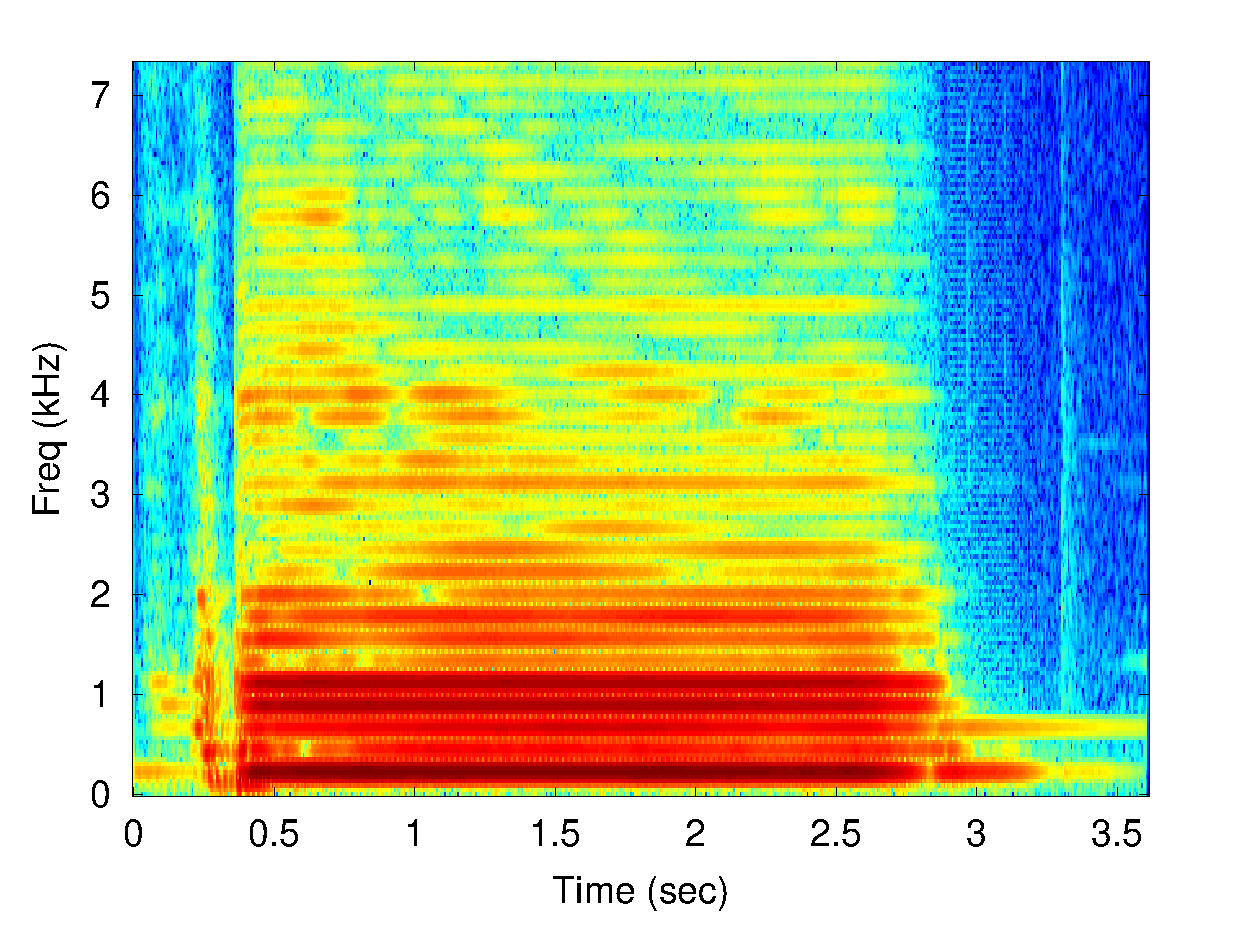
\includegraphics[width=0.45\textwidth]{chapter3/Images/CelloSpectrogram.eps}
				\label{fig:CelloSpectrogram}
			}
			\qquad
			\subfloat[Filtered Sample]
			{
				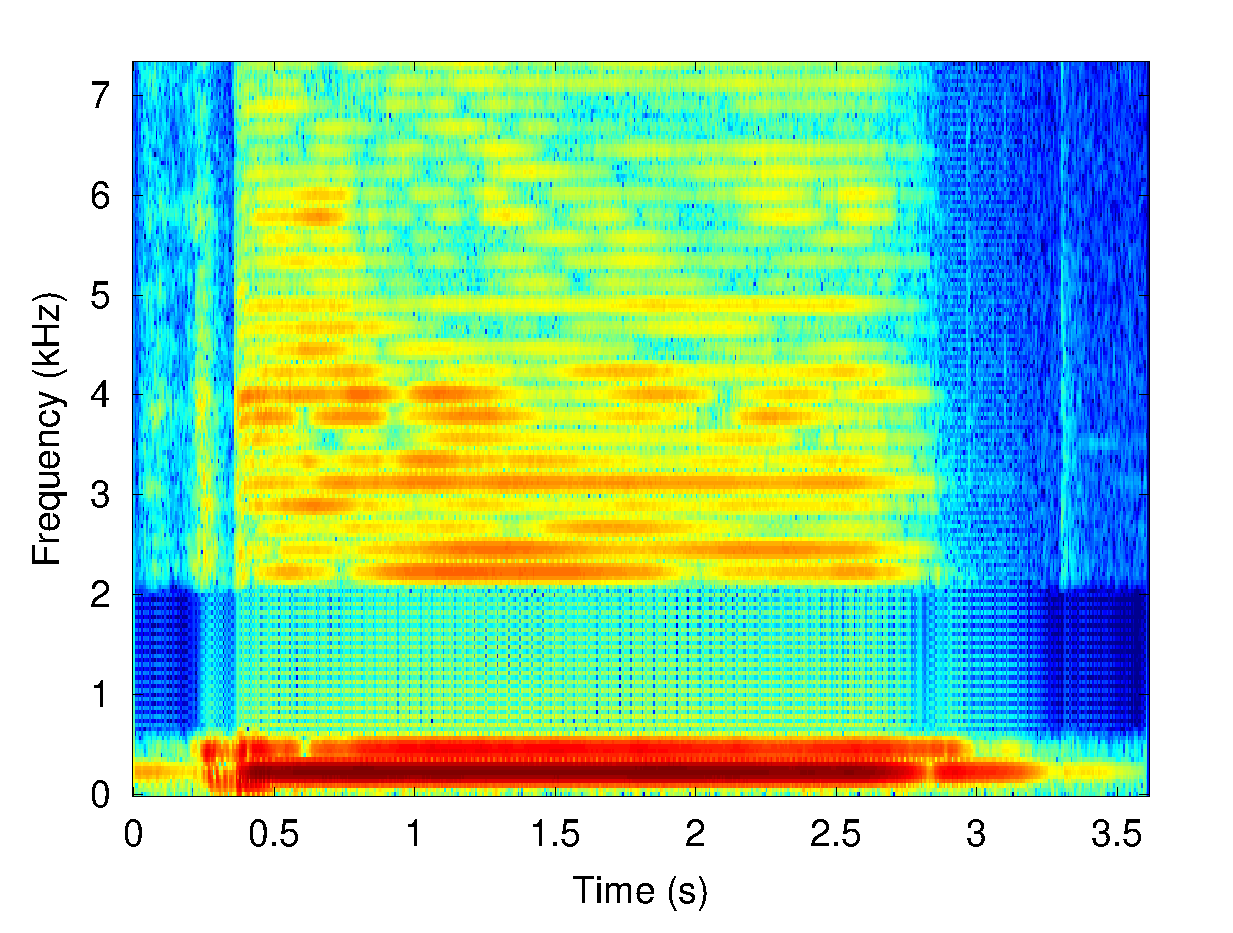
\includegraphics[width=0.45\textwidth]{chapter3/Images/CelloFilteredSpectrogram.eps}
				\label{fig:CelloFilteredSpectrogram}
			}
			\caption{Spectrograms of the cello sample.}
			\label{fig:CelloSpectrograms}
		\end{figure}

		Each sample was reconstructed three times using each method, using different parameters each time. For the
		SSBA and IAP methods a different order FIR filter was used to isolate the fundamental frequency. The
		filters used had orders of 50, 100 and 500. For the synthesis method the window length of the STFT was
		changed, taking values of 50, 100 and 500 samples. Spectrograms for the reconstructed samples using the
		smallest filter order / STFT window length are shown in Figure \ref{fig:ReconstructedCelloSpectrograms}.

		\begin{figure}[h!]
			\centering
			\subfloat[SSBA with a 50\super{th} order filter.]
			{
				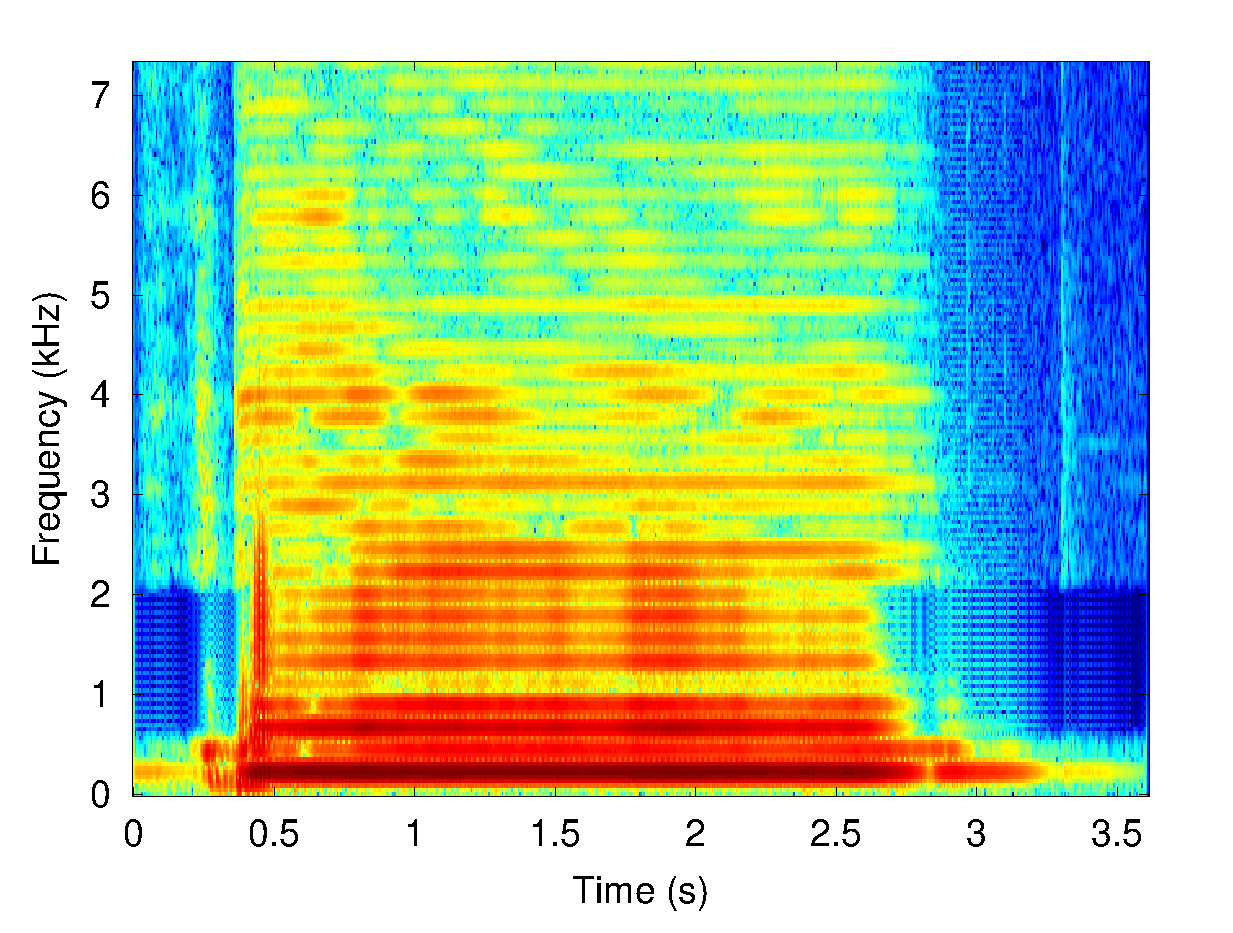
\includegraphics[width=0.45\textwidth]{chapter3/Images/CelloSSBASpectrogram.eps}
				\label{fig:CelloSSBASpectrogram}
			}
			\qquad
			\subfloat[IAP with a 50\super{th} order filter.]
			{
				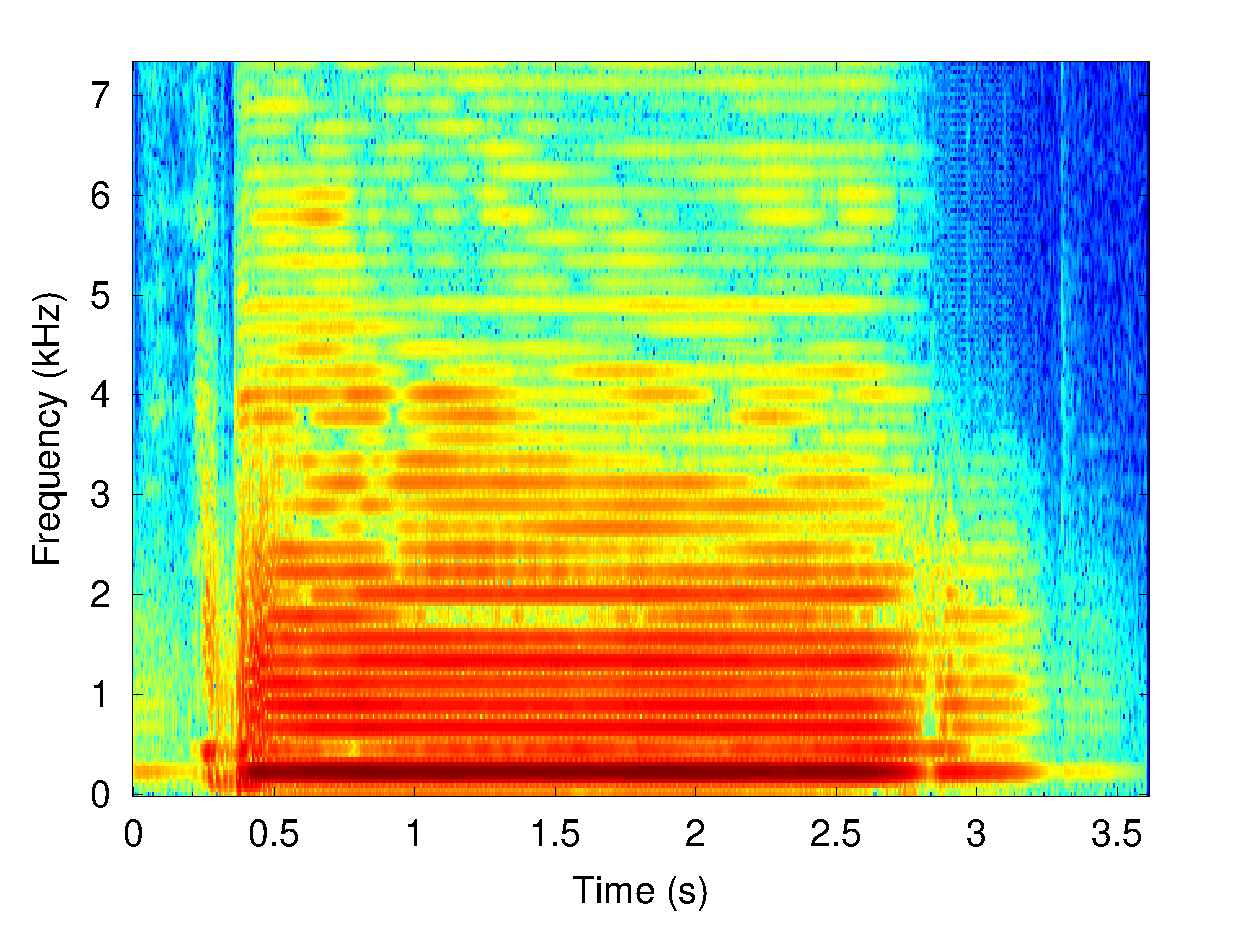
\includegraphics[width=0.45\textwidth]{chapter3/Images/CelloIAPSpectrogram.eps}
				\label{fig:CelloIAPSpectrogram}
			}
			
			\subfloat[Synthesis with an STFT window length of 50 samples.]
			{
				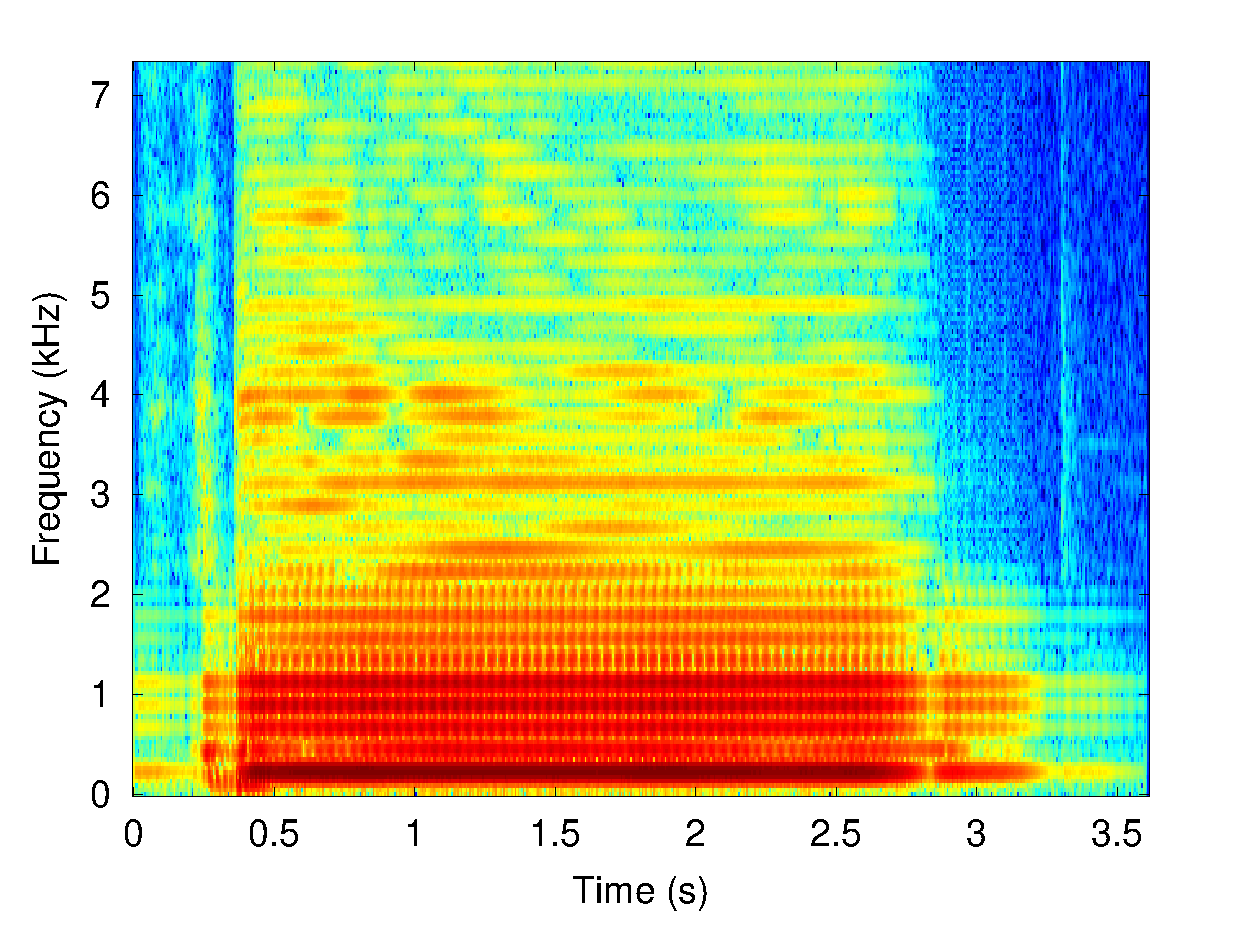
\includegraphics[width=0.45\textwidth]{chapter3/Images/CelloSynthesisSpectrogram.eps}
				\label{fig:CelloSynthesisSpectrogram}
			}
			\caption{Spectrograms of the cello sample reconstructed using three different methods.}
			\label{fig:ReconstructedCelloSpectrograms}
		\end{figure}

		On inspection of these spectrograms the characteristics of the three excitation methods can be seen. The
		amplitude envelopes of the generated harmonics differ greatly between the methods. Comparing the decay
		portion of the envelopes compared with those in the original signal (Figure \ref{fig:CelloSpectrogram})
		highlights these differences. In the cello sample the fundamental frequency and third harmonic have a
		longer decay time then the other harmonics. The harmonics generated by the IAP and synthesis methods
		(Figures \ref{fig:CelloIAPSpectrogram} and \ref{fig:CelloSynthesisSpectrogram}) use the amplitude envelope
		of the fundamental frequency extending the decay time of the these harmonics compared to that in the
		original. Those generated by the SSBA method (Figure \ref{fig:CelloSSBASpectrogram}) have shortened decay
		times. As the order of the harmonic is increased the decay time gets shorter due to the dynamic expansion
		shown in Figure \ref{fig:SSBATemporalEffects}.

		The amplitude envelopes of the harmonics generated using the synthesis techniques exhibit a large amount of
		ripple. This is due to the amplitude of the fundamental being calculated in blocks. These inaccuracies are
		not present in the harmonics generated using the IAP method as the amplitude is calculated on a sample by
		sample basis.

		Test participants were presented with all processed version of a particular sample at once along with a
		reference stimulus (the unprocessed sample) and an anchor stimulus (the sample with its harmonics removed).
		Participants were asked to grade how well each processed stimulus recreated the reference stimulus on a
		scale from 0 to 100.

		The results of this experiment are shown in Figure \ref{fig:SMCResults} with error bars showing the 95\%
		confidence intervals. The stimuli numbers refer to different processing algorithms as follows.

		\begin{tabular}{>{\bfseries}cl}
			1. & Reference Stimulus \\
			2. & Sample reconstructed using the synthesis method with an STFT window length of 50
			     samples. \\
			3. & Sample reconstructed using the synthesis method with an STFT window length of 100
			     samples. \\
			4. & Sample reconstructed using the synthesis method with an STFT window length of 500
			     samples. \\
			5. & Sample Reconstructed using the SSBA method using a 50\super{th} order filter.\\
			6. & Sample Reconstructed using the SSBA method using a 100\super{th} order filter.\\
			7. & Sample Reconstructed using the SSBA method using a 500\super{th} order filter.\\
			8. & Sample Reconstructed using the IAP method using a 50\super{th} order filter.\\
			9. & Sample Reconstructed using the IAP method using a 100\super{th} order filter.\\
		     	10. & Sample Reconstructed using the IAP method using a 500\super{th} order filter.\\
	     		11. & Sample with third through ninth harmonics removed (anchor).\\
		\end{tabular}

		\begin{figure}[h!]
			\centering
			\subfloat[Cello Sample]
			{
				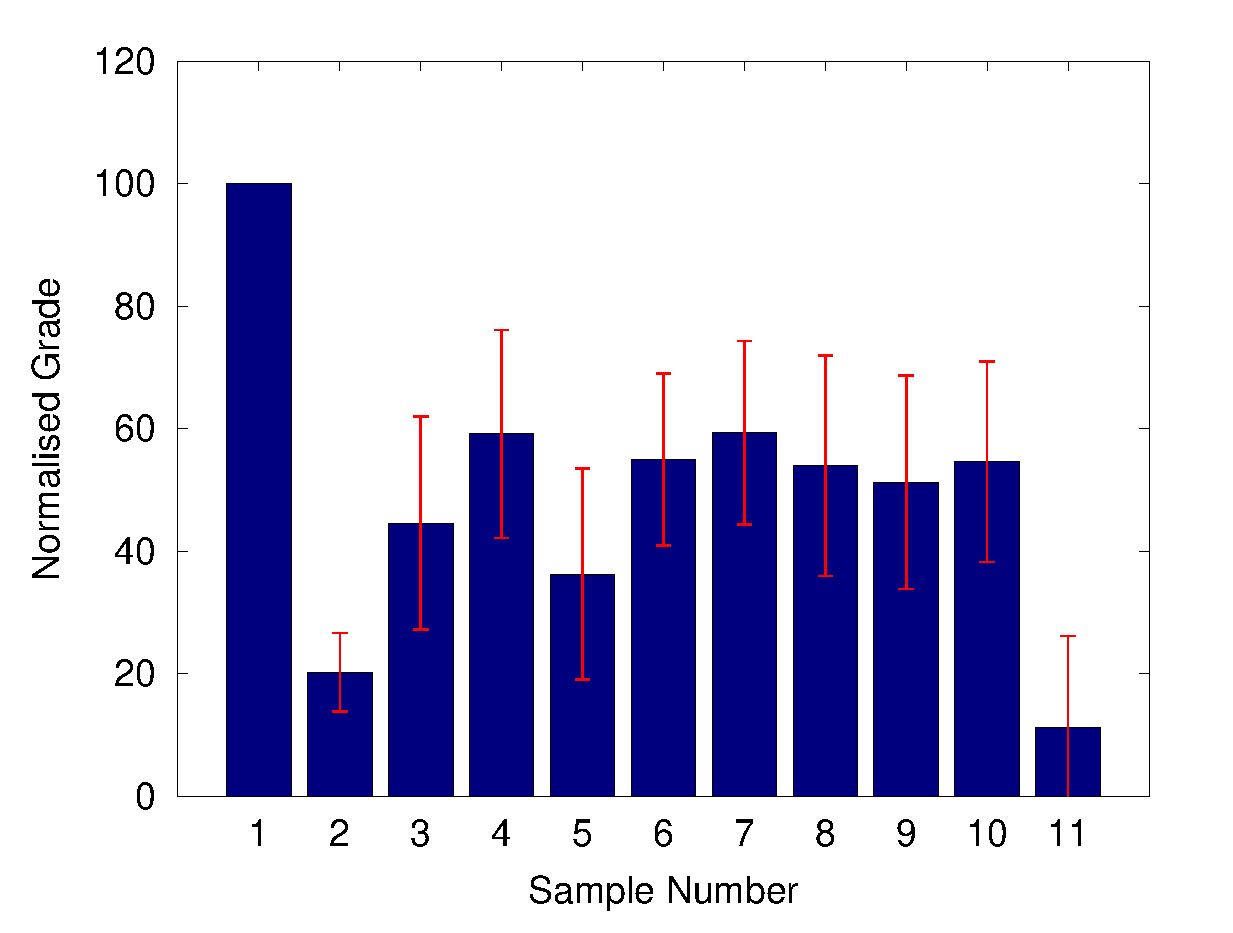
\includegraphics[width=0.45\textwidth]{chapter3/Images/CelloResults.eps}
				\label{fig:CelloResults}
			}
			\qquad
			\subfloat[Clarinet Sample]
			{
				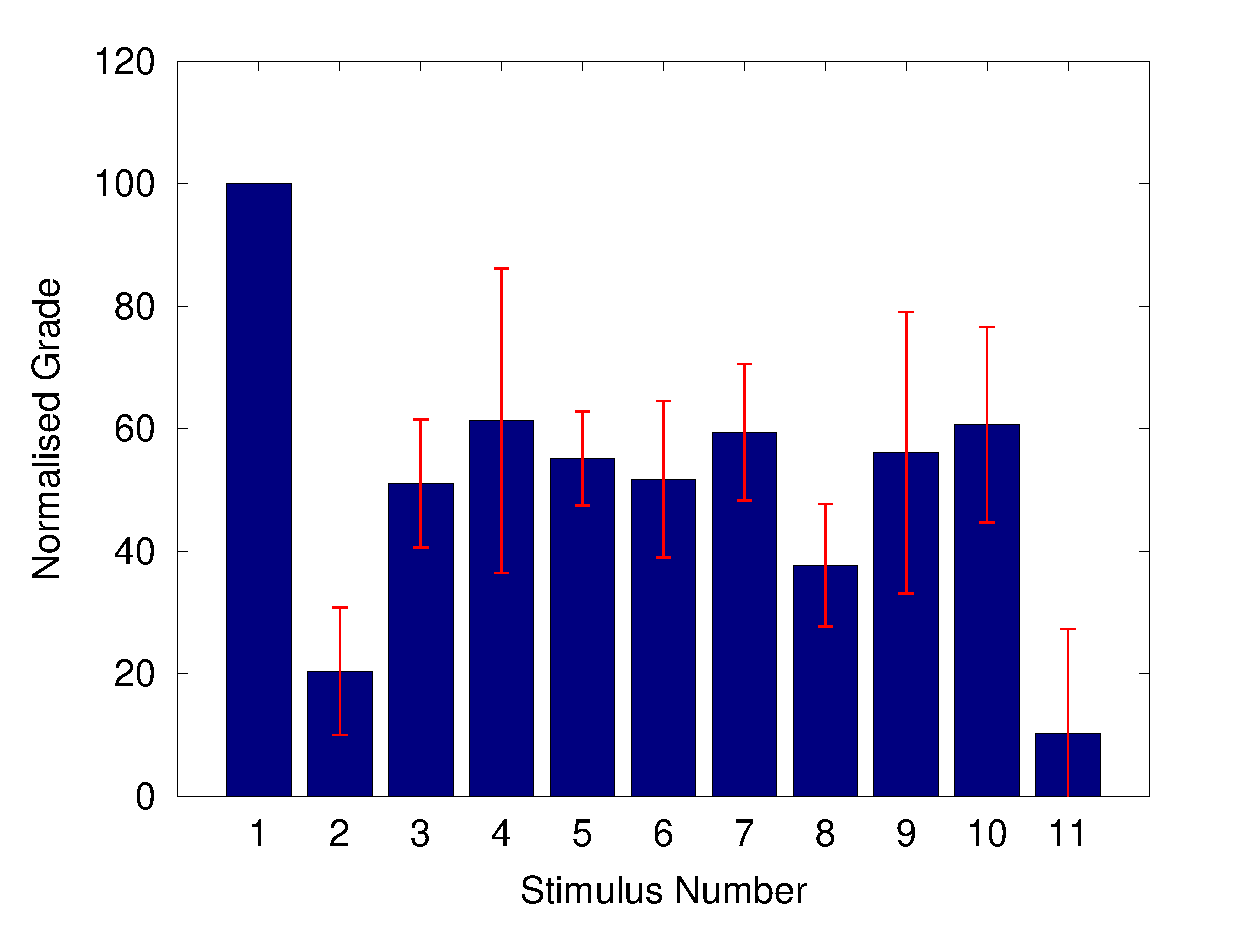
\includegraphics[width=0.45\textwidth]{chapter3/Images/ClarinetResults.eps}
				\label{fig:ClarinetResults}
			}

			\subfloat[Synthesised Sample]
			{
				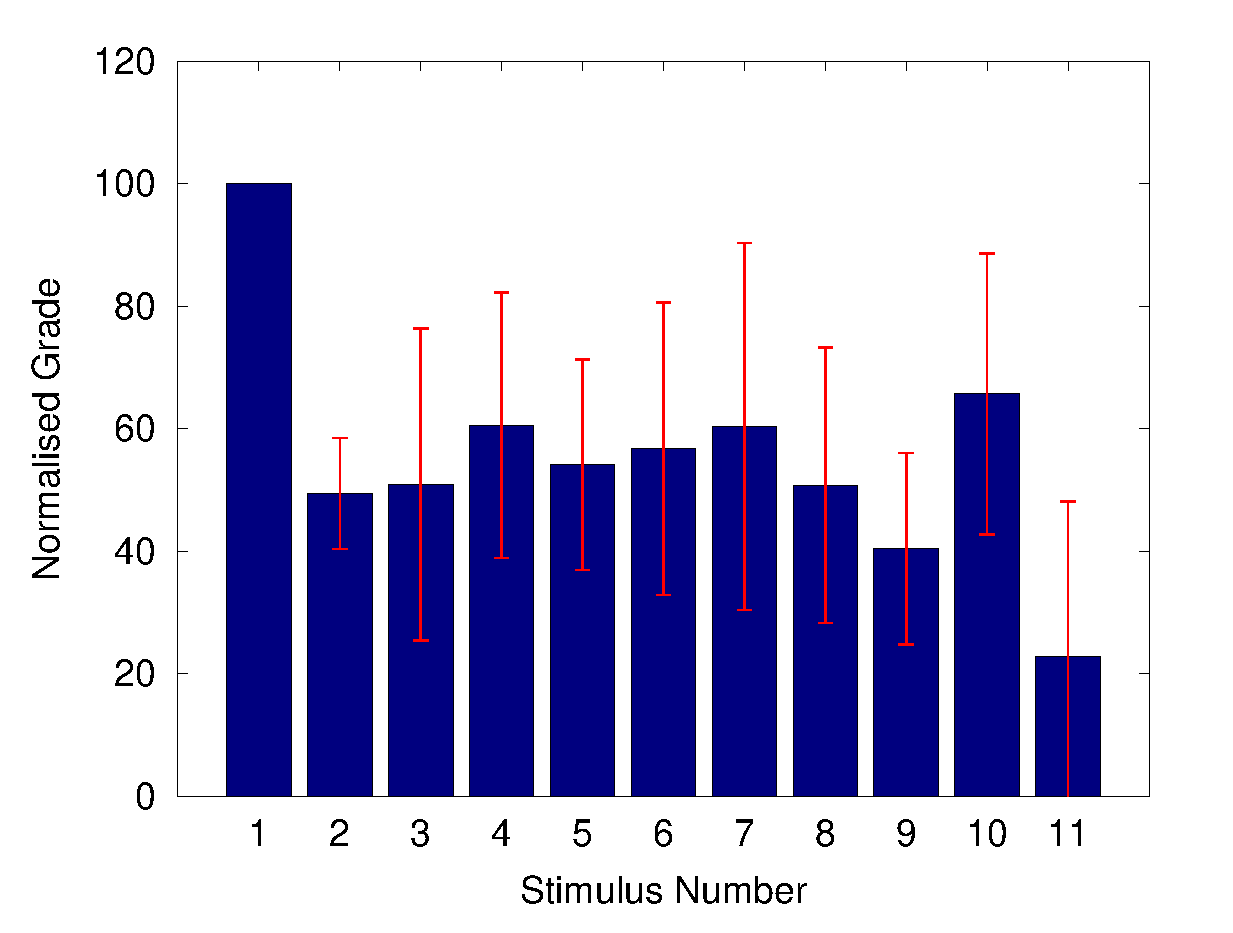
\includegraphics[width=0.45\textwidth]{chapter3/Images/SynthResults.eps}
				\label{fig:SynthResults}
			}
			\qquad
			\subfloat[Piano Sample]
			{
				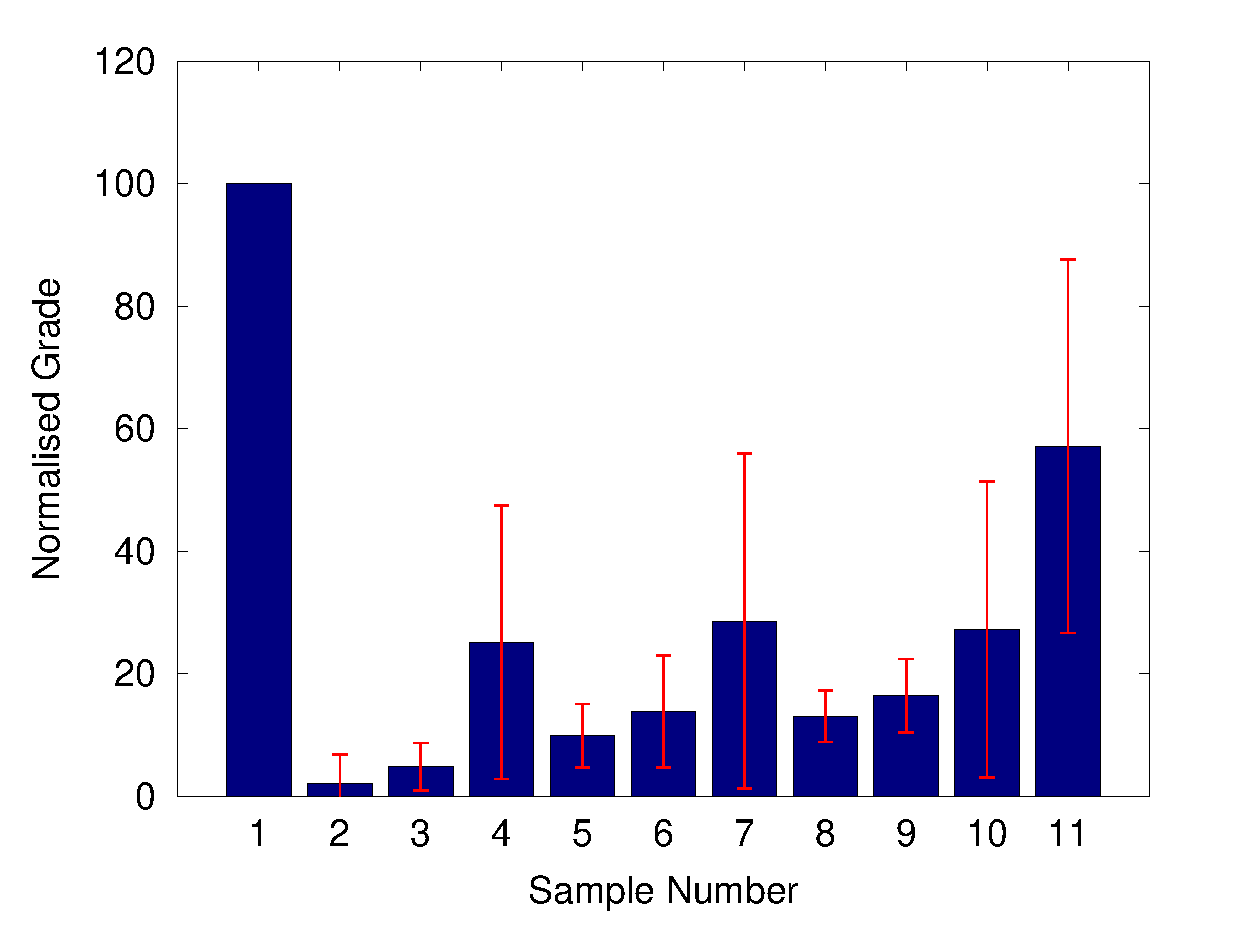
\includegraphics[width=0.45\textwidth]{chapter3/Images/PianoResults.eps}
				\label{fig:PianoResults}
			}
			\caption{Mean grades and confidence intervals for each of the stimuli.}
			\label{fig:SMCResults}
		\end{figure}

		Across all the samples there is a general increase in the perceived quality of the reproduction as the
		filter order or STFT window length is increased. With the SSBA and IAP methods increasing the filter order
		increases the level difference between the fundamental and its harmonics, better isolating the fundamental.
		This is turn reduces the levels of intermodulation distortion in the output producing a `cleaner' harmonic.
		With the synthesis method increasing the STFT window length increases the frequency resolution allowing for
		the amplitude envelope of the fundamental frequency to be measured more precisely.

		The piano sample used had very little energy at its fundamental frequency. This illustrates the problem
		discussed previously, there is not enough information in the amplitude envelope of the fundamental to
		reproduce the other harmonics. This leads to much lower grades for the reproduced signals than for any of
		the other samples. Figure \ref{fig:PianoResults} shows that the piano sample with its harmonics
		missing received a higher grade on average then any of the reconstructed samples further showing how poor
		the quality of the reconstructions is.

		The confidence intervals for the grades given to the majority of the stimuli are high. This is most likely
		due to there being too few participants in the experiment. To supplement these results each of the stimuli
		was graded with the R\sub{nonlin} metric. These results were normalised to the same range as the results
		from the listening test and are displayed in Figure \ref{fig:SMCRNonlin}.

		\begin{figure}[h!]
			\centering
			\subfloat[Cello Sample]
			{
				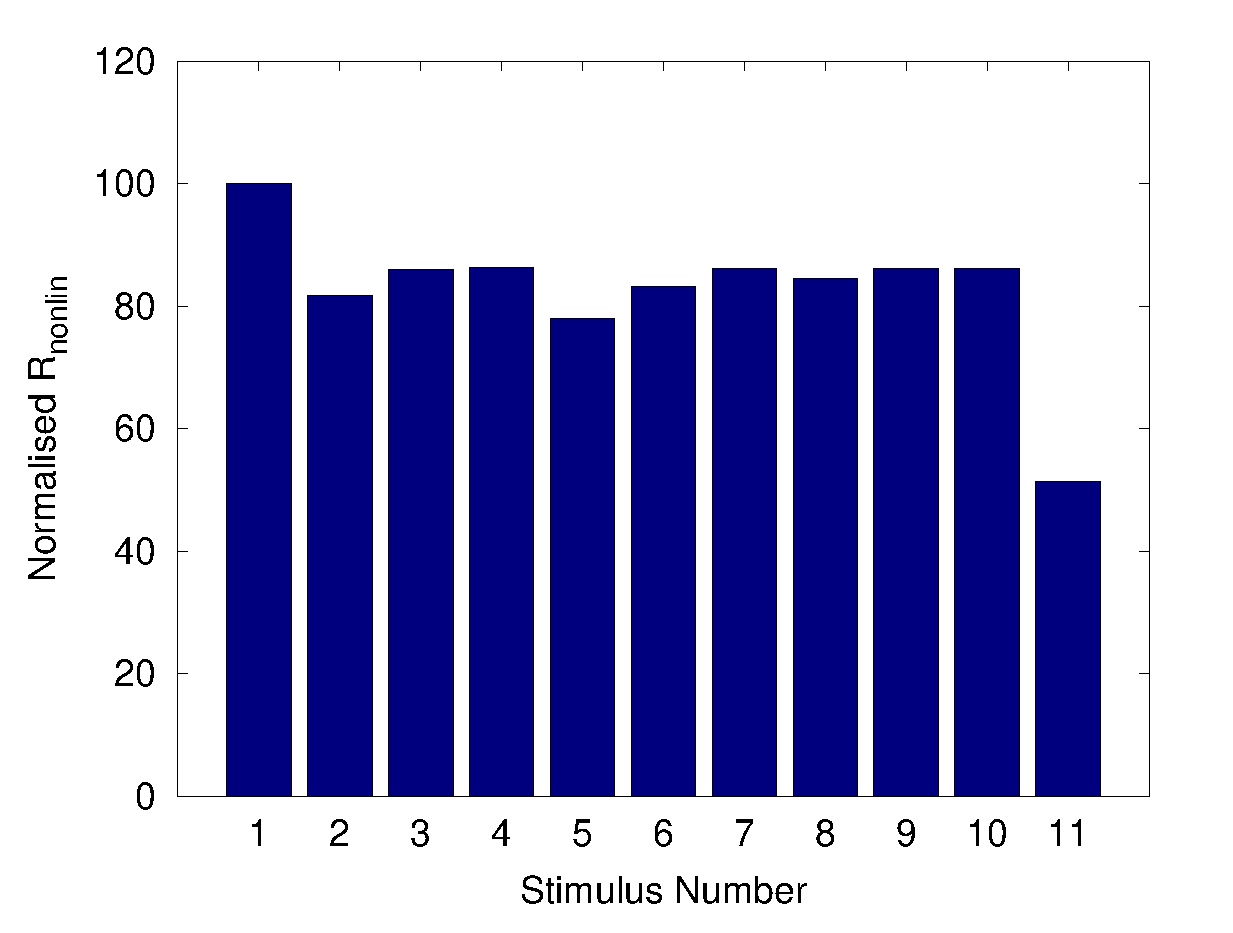
\includegraphics[width=0.45\textwidth]{chapter3/Images/CelloRNonlin.eps}
				\label{fig:CelloRNonlin}
			}
			\qquad
			\subfloat[Clarinet Sample]
			{
				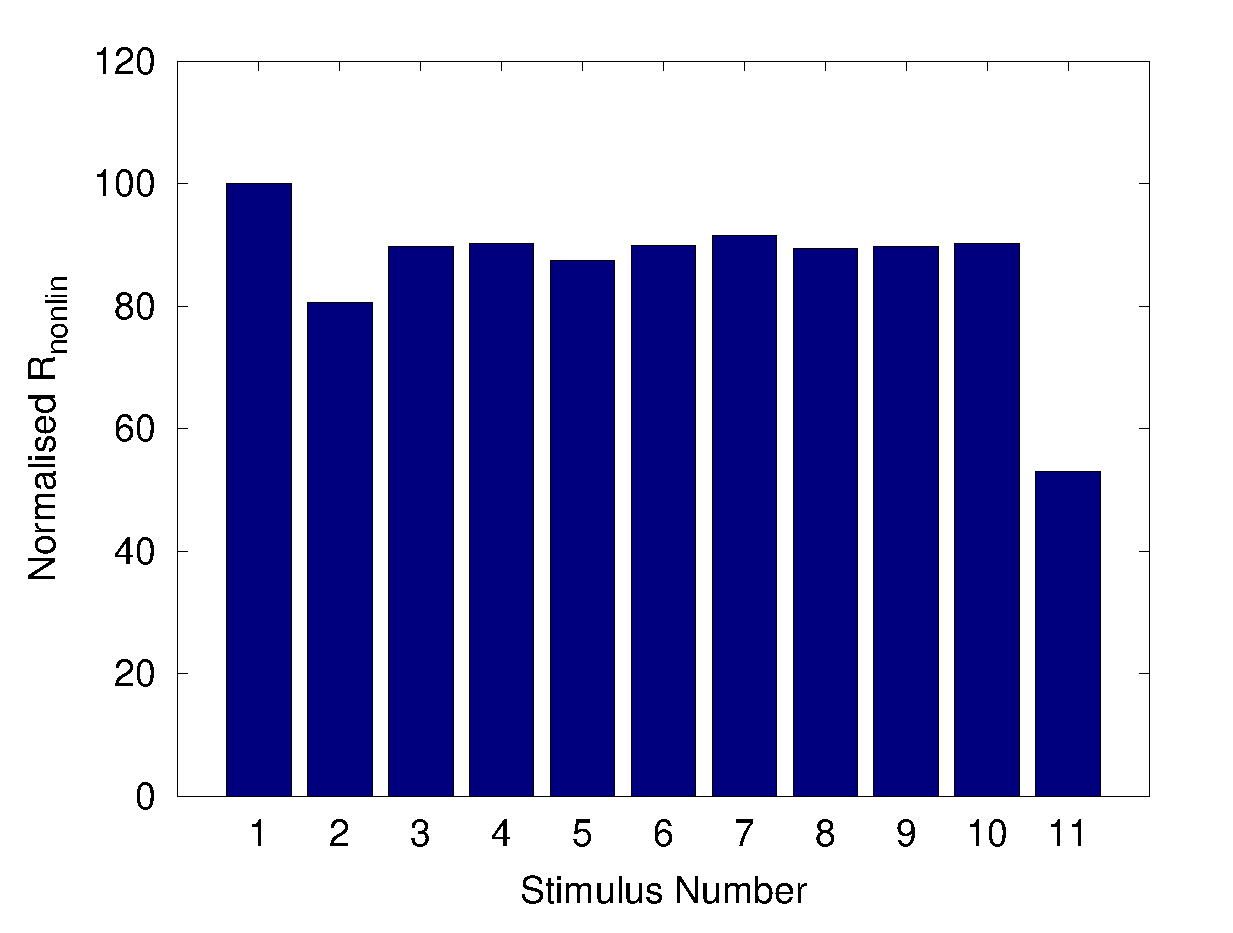
\includegraphics[width=0.45\textwidth]{chapter3/Images/ClarinetRNonlin.eps}
				\label{fig:ClarinetRNonlin}
			}

			\subfloat[Synthesised Sample]
			{
				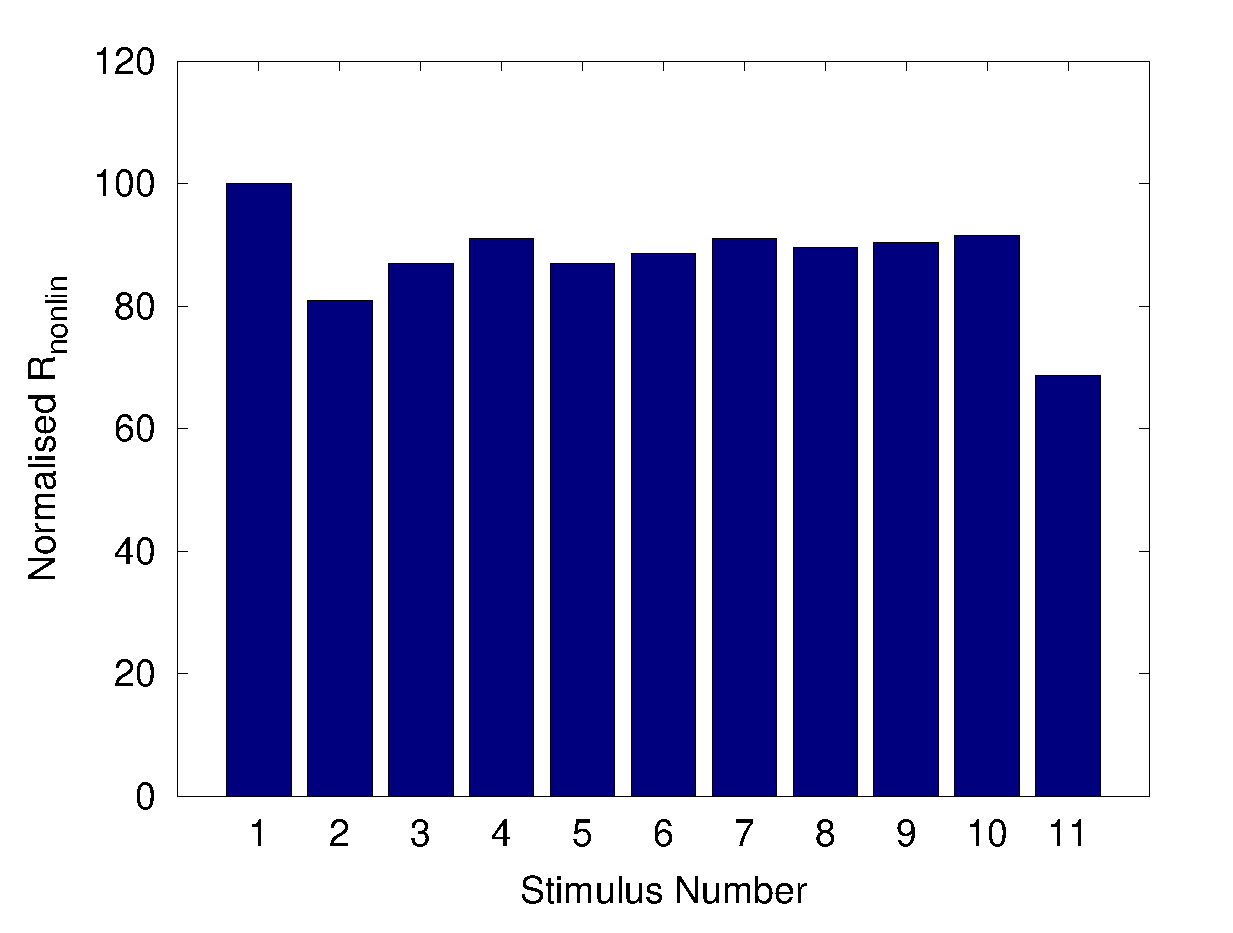
\includegraphics[width=0.45\textwidth]{chapter3/Images/SynthRNonlin.eps}
				\label{fig:SynthRNonlin}
			}
			\qquad
			\subfloat[Piano Sample]
			{
				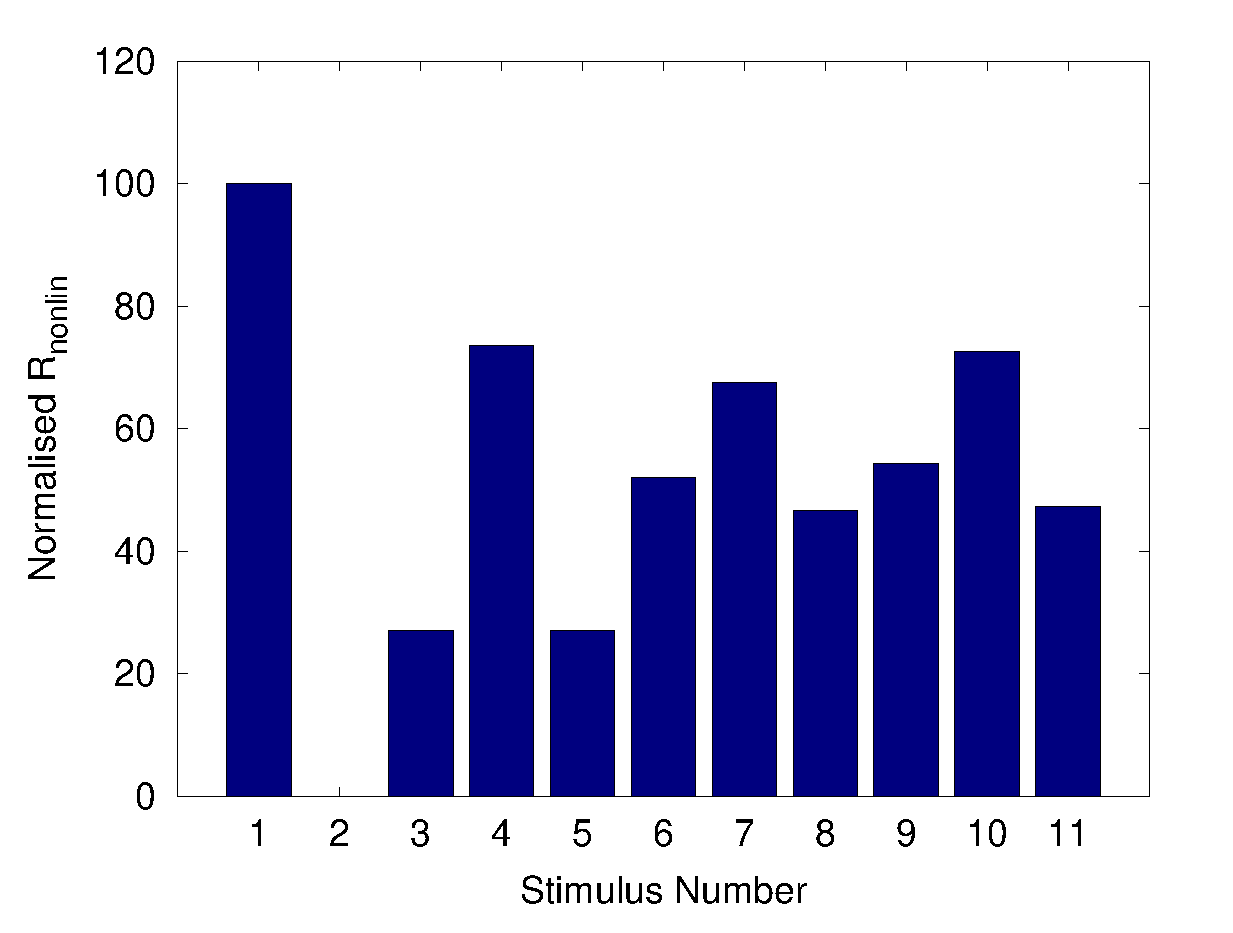
\includegraphics[width=0.45\textwidth]{chapter3/Images/PianoRNonlin.eps}
				\label{fig:PianoRNonlin}
			}
			\caption{R\sub{nonlin} values for each of the stimuli.}
			\label{fig:SMCRNonlin}
		\end{figure}

		The R\sub{nonlin} values support the correlations found in the listening test results. Using a higher order
		filter to isolate the fundamental improves the quality of the reconstruction. Figure \ref{fig:PianoRNonlin}
		again illustrates the problems which arise when the input signal has little energy at its fundamental
		frequency. Several of the reconstructions are objectively less similar to the original signal than the
		anchor stimulus.

		Both sets of results show that, using the highest order filter / STFT window lengths, each of the methods
		produce similar quality reconstructions of the original signal. For shorter filter lengths the IAP method
		provides more quality at then the SSBA method at the expense of requiring slightly more computation. The
		synthesis method produces similar quality results but incurs further computational complexity. 
		
		For timbral control applications the IAP method provides the greatest flexibility. For the majority of
		stimuli in this experiment it reproduced signals with the highest perceived quality. It was also shown in
		section \ref{sec:FeatureControl-IAP} that it is a homogeneous process allowing it to be applied to a wider
		range of signals with more predictable effects.

\section{Controlling features with Exciters}
\label{sec:FeatureControl-Control}
